\PassOptionsToPackage{inline,shortlabels}{enumitem}
\documentclass[12pt, oneside, a4paper, english, brazil]{abntex2}

\usepackage[logohorizontal, CAR]{abntex2-ifsp} 
% ---
		
% ---
\usepackage{amsmath}
\usepackage{amsfonts}
\usepackage{amssymb}
\usepackage{amsthm}

\usepackage{xpatch}

\usepackage{enumerate} 
\usepackage{graphicx}
\usepackage{tikz}



\providecommand{\abs}[1]{\left\vert #1 \right\vert}
\providecommand{\p}[1]{\left( #1 \right)}
\providecommand{\chaves}[1]{\left\{ #1 \right\}}
\providecommand{\colchetes}[1]{\left[ #1 \right]}
\providecommand{\Endo}[1]{\text{End}\left( #1 \right)}
\providecommand{\Endor}[1]{\text{End}_{\mathbb{R}}\left( #1 \right)}


\providecommand{\R}{\mathbb{R}}
\providecommand{\Rdois}{\mathbb{R}^2}
\providecommand{\Rtres}{\mathbb{R}^3}
\newcommand{\C}{\mathbb{C}}
%\newcommand{\bs}{\backslash}
\newcommand{\vep}{\varepsilon}
\providecommand{\rad}{\text{ rad}}

\providecommand{\ac}{Álgebras de Clifford}
\providecommand{\Cl}{\mathcal{C}\ell}
\providecommand{\Cldois}{\mathcal{C}\ell_2}
\providecommand{\Cldoispar}{\mathcal{C}\ell_2^{+}}
\providecommand{\Cldoisimpar}{\mathcal{C}\ell_2^{-}}

\providecommand{\pref}[1]{(\ref{#1})}
\providecommand{\bref}[1]{[\ref{#1}]}

\renewcommand{\vec}{\overrightarrow}
\renewcommand{\qedsymbol}{$\blacksquare$}

% ---

% ---
% Definições, Teoremas, Corolários ...
% ---
\providecommand{\definitionref}[1]{[Definição \ref{#1}]}
\providecommand{\propositionref}[1]{[Proposição \ref{#1}]}
\providecommand{\propertyref}[1]{[Propriedade \ref{#1}]}
\providecommand{\observationref}[1]{[Observação \ref{#1}]}
\providecommand{\corollaryref}[1]{[Corolário \ref{#1}]}
\providecommand{\lemmaref}[1]{[Lema \ref{#1}]}
\providecommand{\theoremref}[1]{[Teorema \ref{#1}]}
\providecommand{\conjectureref}[1]{[Conjectura \ref{#1}]}
\providecommand{\exempleref}[1]{[Exemplo \ref{#1}]}
\providecommand{\notationref}[1]{[Notação \ref{#1}]}

\xpatchcmd{\proof}{\hskip\labelsep}{\hskip6.5\labelsep}{}{}

\newtheoremstyle{normal}% name
{}% Space above1
{}% Space below1
{}% Body font
{\parindent}% Indent amount2
{\bfseries}% Theorem head font
{.}% Punctuation after theorem head
{ }% Space after theorem head3
{}% Theorem head spec (can be left empty, meaning ‘normal’)

\newtheoremstyle{observacao} 
{}% Space above1
{}% Space below1
{}% Body font
{\parindent}% Indent amount2
{\bfseries}% Theorem head font
{:}% Punctuation after theorem head
{ }% Space after theorem head3
{}% Theorem head spec (can be left empty, meaning ‘normal’)


\newcounter{geral}

\theoremstyle{normal}
\newtheorem{definition}[geral]{Definição}
\newtheorem{proposition}[geral]{Proposição}
\newtheorem{property}[geral]{Propriedade}
\newtheorem{corollary}[geral]{Corolário}
\newtheorem{lemma}[geral]{Lema}
\newtheorem{theorem}[geral]{Teorema}
\newtheorem{conjecture}[geral]{Conjectura}
\newtheorem{notation}[geral]{Notação}
\newtheorem{vocabulary}[geral]{Vocabulário}

\theoremstyle{observacao}
\newtheorem*{obs}{Observação}


% ---
% Informações de dados para CAPA e FOLHA DE ROSTO
% ---
\titulo{As Álgebras de Clifford}
\autor{Marcio Oliveira de Morais Junior}
%\local{Brasil}
\data{2016}
\datadefesa{\today}
\orientador{Prof. Me. Márcio André Traesel}
%\coorientador{Um coorientador}
\membrobancaA{Prof. Me. }
\membrobancaB{Prof. Me. }


\tipotrabalho{Trabalho de Conclusão de Curso}
\preambulo{Monografia submetida ao Instituto Federal de Educação, Ciência e Tecnologia de São Paulo -- Câmpus Caraguatatuba como parte dos requisitos para obtenção do grau de Licenciado em Matemática.}
% ---


% ---
% Configurações de aparência do PDF final

% alterando o aspecto da cor azul
\definecolor{blue}{RGB}{41,5,195}

% informações do PDF
\makeatletter
\hypersetup{
%pagebackref=true,
pdftitle={\@title}, 
pdfauthor={\@author},
pdfsubject={\imprimirpreambulo},
pdfcreator={LaTeX with abnTeX2},
pdfkeywords={Álgebras de Clifford}{Álgebras Geométricas}{Matemática Pura}{Matemática Aplicada}, 
colorlinks=false,       		% false: boxed links; true: colored links
linkcolor=blue,          	% color of internal links
citecolor=blue,        		% color of links to bibliography
filecolor=magenta,      	% color of file links
urlcolor=blue,
bookmarksdepth=4
}
\makeatother
% --- 

% ---
% compila o indice
% ---
\makeindex
% ---

% ----------------------------------------------------------
% Início do documento
% ----------------------------------------------------------
\begin{document}

% ----------------------------------------------------------
% ELEMENTOS PRÉ-TEXTUAIS
% ----------------------------------------------------------
\pretextual

% ----------------------------------------------------------
% Capa
% ----------------------------------------------------------
\imprimircapa


% ----------------------------------------------------------
% Folha de rosto
% (o * indica que haverá a ficha bibliográfica)
% ----------------------------------------------------------
\imprimirfolhaderosto*


% ----------------------------------------------------------
% Inserir a ficha bibliografica
% ----------------------------------------------------------

% Isto é um exemplo de Ficha Catalográfica, ou ``Dados internacionais de
% catalogação-na-publicação''. Você pode utilizar este modelo como referência. 
% Porém, provavelmente a biblioteca da seu câmpus lhe fornecerá um PDF
% com a ficha catalográfica definitiva após a defesa do trabalho. Quando estiver
% com o documento, salve-o como PDF no diretório do seu projeto e substitua todo
% o conteúdo de implementação deste arquivo pelo comando abaixo:
%
% \begin{fichacatalografica}
%     \includepdf{fichacatalografica.pdf}
% \end{fichacatalografica}
\begin{fichacatalografica}
\vspace*{\fill}					% Posição vertical
\hrule							% Linha horizontal
\begin{center}					% Minipage Centralizado
\begin{minipage}[c]{12.5cm}		% Largura

\imprimirautor

\hspace{0.5cm} \imprimirtitulo  / \imprimirautor. --
\imprimirlocal, \imprimirdata-

\hspace{0.5cm} \pageref{LastPage} p. : il. (algumas color.) ; 30 cm.\\

\hspace{0.5cm} \imprimirorientadorRotulo~\imprimirorientador\\

\hspace{0.5cm}
\parbox[t]{\textwidth}{\imprimirtipotrabalho~--~\imprimirinstituicao,
\imprimirdata.}\\

\hspace{0.5cm}
1. Palavra-chave1.
2. Palavra-chave2.
I. Orientador.
II. Universidade xxx.
III. Faculdade de xxx.
IV. Título\\ 			
	
\hspace{8.75cm} CDU 02:141:005.7\\
	
\end{minipage}
\end{center}
\hrule
\end{fichacatalografica}


% ----------------------------------------------------------
% Inserir errata
% ----------------------------------------------------------
%\begin{errata}
%Elemento opcional da \citeonline[4.2.1.2]{NBR14724:2011}. Exemplo:
%
%\vspace{\onelineskip}
%
%FERRIGNO, C. R. A. \textbf{Tratamento de neoplasias ósseas apendiculares com
%reimplantação de enxerto ósseo autólogo autoclavado associado ao plasma
%rico em plaquetas}: estudo crítico na cirurgia de preservação de membro em
%cães. 2011. 128 f. Tese (Livre-Docência) - Faculdade de Medicina Veterinária e
%Zootecnia, Universidade de São Paulo, São Paulo, 2011.
%
%\begin{table}[htb]
%\center
%\footnotesize
%\begin{tabular}{p{1.4cm}|p{1cm}|p{3cm}|p{3cm}}
%\hline
%\textbf{Folha} & \textbf{Linha}  & \textbf{Onde se lê}  & \textbf{Leia-se}  \\
%\hline
%1 & 10 & auto-conclavo & autoconclavo\\
%\hline
%\end{tabular}
%\end{table}
%\end{errata}


% ----------------------------------------------------------
% Inserir folha de aprovação
% ----------------------------------------------------------

% Isto é um exemplo de Folha de aprovação, elemento obrigatório da NBR
% 14724/2011 (seção 4.2.1.3). Você pode utilizar este modelo até a aprovação
% do trabalho. Após isso, substitua todo o conteúdo deste arquivo por uma
% imagem da página assinada pela banca com o comando abaixo:
%
% \includepdf{folhadeaprovacao_final.pdf}
%
% Sugestão: Imprima uma cópia desta página e não encaderne-a, assim fica 
% mais fácil escaneá-la para gerar um pdf

\imprimefolhadeaprovacao


% ----------------------------------------------------------
% Dedicatória
% ----------------------------------------------------------
\begin{dedicatoria}
\vspace*{\fill}
\hspace{.24\textwidth}
\begin{minipage}{.7\textwidth}
\flushright
\noindent
\textit{Àqueles que um dia viajaram e deslumbraram \\
a beleza matemática.}
\end{minipage}
\end{dedicatoria}
%\imprimirdedicatoria

% ----------------------------------------------------------
% Agradecimentos
% ----------------------------------------------------------
\begin{agradecimentos}

\end{agradecimentos}


% ----------------------------------------------------------
% Epígrafe
% ----------------------------------------------------------
\begin{epigrafe}
\vspace*{\fill}
\hspace{.24\textwidth}
\begin{minipage}{.7\textwidth}
\flushright
\noindent
\textit{``Digno és, Jeová, nosso Deus, de receber a glória, a honra e o poder, porque criaste todas as coisas, e por tua vontade elas vieram à existência e foram criadas.''\\
(Apocalipse 4: 11)}
\end{minipage}
\end{epigrafe}


% ----------------------------------------------------------
% RESUMOS
% ----------------------------------------------------------

% resumo em português
\begin{resumo}


\vspace{\onelineskip}

\noindent
\textbf{Palavras-chaves}: Álgebras de Clifford. Álgebras Geométricas. Produto Exterior.
\end{resumo}

% resumo em inglês
\begin{resumo}[Abstract]
\begin{otherlanguage*}{english}
This is the english abstract.

\vspace{\onelineskip}
 
\noindent 
\textbf{Key-words}: Clifford Algebras. Geometric Algebras. Exterior Product.
\end{otherlanguage*}
\end{resumo}
% ---

% ---
% inserir lista de ilustrações
% ---
\pdfbookmark[0]{\listfigurename}{lof}
\listoffigures*
\newpage
% ---

% ---
% inserir lista de tabelas
% ---
\pdfbookmark[0]{\listtablename}{lot}
\listoftables*
\newpage
% ---

% ---
% inserir lista de abreviaturas e siglas
% ---
\begin{siglas}
\item[i. e.] \textit{id est} (isto é)
\end{siglas}
% ---

% ---
% inserir lista de símbolos
% ---
\begin{simbolos}
\item[$\Cldois$] Álgebra de Clifford
\item[$\Cldoispar$] Parte par de $\Cldois$
\item[$\Cldoisimpar$] Parte ímpar de $\Cldois$
\item[$\Cl_n$] 
\end{simbolos}
% ---

% ---
% inserir o sumario
% ---
\pdfbookmark[0]{\contentsname}{toc}
\tableofcontents*
\cleardoublepage
% ---


% ----------------------------------------------------------
% ELEMENTOS TEXTUAIS
% ----------------------------------------------------------
\textual
\pagestyle{simple}

\chapter{Introdução}

ATENÇÃO: A introdução ainda não concluída.

Muito se tem estudado sobre as álgebras de Clifford. Entretanto, boa parte desses estudos são dedicadas à aplicações dessas álgebras na física-matemática e não trazem em seu escopo os conceitos básicos de tal álgebra. (Referenciar)

Assim, este trabalho tem por objetivo realizar um levantamento bibliográfico e apresentar de maneira clara e concisa os fundamentos para a compreensão das álgebras de Clifford, com linguagem acessível aos estudantes de graduação.


O capítulo \ref{algebrasgeometricas}, tratará principalmente sobre o contexto histórico do desenvolvimento das \ac. 

O capítulo \ref{revisao} é baseado em \citeonline{lounesto2001}, \citeonline{winterle2000} e \citeonline{callioli1990} e traz brevemente os principais conceitos necessários para uma melhor compreensão do capítulo \ref{clifford}. 

O capítulo \ref{complexos} tem por objetivo abordar o corpo dos complexos ($\C$) afim de, no capítulo \ref{partesdecl2}, ampliar a compreensão do capítulo \ref{clifford}.

\chapter{Álgebras Geométricas}\label{algebrasgeometricas}
Hoje lemos ``\emph{xis ao quadrado}'' e ``\emph{xis ao cubo}'' ao ler $x^2$ e $x^3$ respectivamente, isso decorre da representação de $x$ como lado de um quadrado, assim a área desse quadrado é dada por $x^2$, da mesma maneira, para $x$ como lado de um cubo, assim o volume desse cubo é dado por $x^3$. Por detrás dessa leitura, há ma ideia muito profunda: a ideia de representar os objetos geométricos por meio de objetos algébricos, bem como as operações geométricas por operações algébricas. Essa ideia remota aos gregos, porém eles não conseguiam representar qualquer segmento de reta. Sabe-se que a decadência da Escola Pitagórica dá-se pela resistência de Pitágoras em reconhecer a diagonal de um quadrado de lado unitário. Dessa maneira, os gregos não poderiam representar qualquer segmento sem o que hoje são chamados de números irracionais. Além disso, como havia apenas a ideia de no máximo o espaço tridimensional, os gregos também não poderiam interpretar geometricamente $x^4$, $x^5$ e assim sucessivamente. \cite{vazjrweb}

A ideia de representar os objetos geométricos por meio de objetos algébricos, bem como as operações geométricas por operações algébricas é o que denominamos \emph{álgebra geométrica}. 

Descartes também tentou estabelecer uma álgebra geométrica, porém não obteve exito. Isso porque para Descates, como para os gregos, bastava dois segmentos de reta terem o mesmo comprimento para serem congruentes. \cite{vazjrweb}

Ao utilizar uma noção de congruência diferente dos gregos, o matemático H. Grassmann, em 1844, conseguiu desenvolver a ideia de uma álgebra geométrica. O grande passo de Grassmann foi utilizar o conceito de vetores para representar segmentos de reta. Com o uso de vetores podemos representar o segmento de reta não somente por seu comprimento mas também por uma orientação e direção. Grassmann definiu o produto exterior de dois vetores, produto que descreve fragmentos de plano. Hoje denominamos a estrutura desenvolvida por Grassmann de álgebra exterior ou álgebra de Grassmann. \cite{vazjr2000}

Também em 1844, W. Hamilton publicou um sistema denominado quatérnions que consistem em uma generalização dos números complexos, que são uma generalização do conceito de números reais. Os quatérnions se mostram adequados para descrever operações no espaço tridimensional. \cite{sousa2013}

Em 1878, Clifford publica um trabalho em que unifica em uma única estrutura os trabalhos de Hamilton e Grassman \cite{sousa2013}. Clifford denomina essa estrutura como álgebra geométrica, mas, atualmente, a denominamos de álgebra de Clifford \cite{vazjr2000}. Assim, as álgebras de Clifford se mostram importantes para o estudo da geometria.  \cite{batistasantos2012}

\section{Os Quatérnions de Hamilton}

\section{O Produto Exterior de Grassmann}

\chapter{Escalares e Vetores}\label{revisao}

Existem dois tipos de grandezas as grandezas escalares e as grandezas vetoriais. Um escalar é uma grandeza que é completamente determinada por seu módulo (intensidade) medido em unidades de uma escala. Um vetor é uma grandeza que é determinada por sua direção, sentido e intensidade. 

Denotamos os vetores por letras sob uma seta ($\vec{a}, \vec{b}, \vec{c}, \ldots$) e o representamos por uma seta. O módulo de um vetor $\vec{a}$ é denotado por $\abs{\vec{a}}$. 

Dois vetores são paralelos se, e somente se, os seus representantes tiverem a mesma direção. 

Na figura acima temos $\vec{a}$ paralelo ao $\vec{b}$ e $\vec{c}$ e indica-se $\vec{a} // \vec{b} // \vec{c}$

Dois vetores são iguais se, e somente se, tem os mesmos módulo, direção e sentido. Então,
\[
\vec{a}=\vec{b} \Longleftrightarrow \abs{\vec{a}}=\abs{\vec{b}} \textrm{ e } \vec{a} \uparrow\uparrow \vec{b}
\]

O vetor nulo tem módulo zero e sua direção e sentido não definidos e é representado por $\vec{0}$. Como este vetor não possuir direção e sentido definidos, considera-se o vetor nulo paralelo a qualquer vetor. 

Para todo vetor não nulo $\vec{a}$ existe um vetor oposto $-\vec{a}$ de mesmo módulo e direção mas sentido oposto.

Um vetor $\vec{a}$ é unitário se $\abs{\vec{a}}=1$. A cada vetor $\vec{b}$, $\vec{b} \neq 0$, é possível associar dois vetores $\vec{a}$ e $-\vec{a}$ de mesma direção de $\vec{b}$. O vetor $\vec{a}$ que tem o mesmo sentido de $\vec{b}$ é chamado versor de $\vec{b}$ e de todos os vetores paralelos e de mesmo sentido de $\vec{b}$. 

Dois vetores são ortogonais algum de seus representantes formam um ângulo reto entre si. Para $\vec{a}$ ortogonal a $\vec{b}$, indica-se $\vec{a} \bot \vec{b}$. Considera-se o vetor nulo ortogonal a qualquer vetor.

Vetores são coplanares se existir algum plano onde esses vetores estão representados. Dois vetores quais quer são sempre coplanares.

\section{Adição e subtração de vetores}

Dados dois vetores $\vec{a}$ e $\vec{b}$, coloque o ponto inicial de $\vec{b}$ no ponto final de $\vec{a}$, a soma $\vec{a} + \vec{b}$ é o vetor com ponto inicial no ponto inicial de $\vec{a}$ e ponto final no ponto final de $\vec{b}$. O vetor soma pode ser visualizada formando um triangulo de lados  $\vec{a}$, $\vec{b}$ e $\vec{a} + \vec{b}$.

Para a soma vetorial, são válidas:
\begin{enumerate}
\item $\vec{a} + \vec{b} = \vec{b}+\vec{a}$ (comutatividade)
\item $(\vec{a} + \vec{b})+\vec{c}=\vec{a} + (\vec{b}+\vec{c})$ (associatividade)
\item $\vec{a} + \vec{0} = \vec{a}$ (elemento neutro)
\item $\vec{a} + (-\vec{a}) = \vec{0}$ (elemento oposto)
\end{enumerate}

O vetor $\vec{a} + (-\vec{b})$, escreve-se $\vec{a}-\vec{b}$, é chamado diferença entre $\vec{a}$ e $\vec{b}$ 

\section{Multiplicação por um número (escalar)}

Seja um número real $\lambda \neq 0$ e $\vec{a}$ um vetor não nulo, chama-se produto do número real $\lambda$ pelo vetor $\vec{a}$, o vetor $\lambda \vec{a}$ tal que:
\begin{enumerate}
\item módulo: $\abs{\lambda\vec{a}} = \abs{\lambda}\abs{\vec{a}}$
\item direção: $\lambda\vec{a}$ é paralelo a $\vec{a}$
\item sentido: 
\begin{align*}
\lambda\vec{a} \uparrow \uparrow \vec{a} &\text{ se } \lambda > 0 \\
\lambda\vec{a} \uparrow \downarrow \vec{a} &\text{ se } \lambda < 0 
\end{align*}
\end{enumerate}

Números que multiplicam vetores são chamados escalares. Para a multiplicação escalar, ou multiplicação por escalar, são válidas ($\forall \lambda, \mu \in \mathbb{R}$ e $\vec{a}, \vec{b}$ vetores)

\begin{enumerate}
\item $\lambda(\vec{a}+\vec{b}) = \lambda\vec{a}+\lambda\vec{b}$, $(\lambda+\mu)\vec{a}= \lambda\vec{a}+\mu\vec{a}$ (distributividade)
\item $(\lambda\mu)\vec{a}=\lambda(\mu\vec{a})$ (associatividade)
\item $1\vec{a} = \vec{a}$
\end{enumerate}

\section{Bases e coordenadas}

No plano, qualquer dois vetores não paralelos $\vec{e_1}$, $\vec{e_2}$ formam uma base de modo que um vetor arbitrário no plano pode ser unicamente expresso como uma combinação linear $\vec{a}= a_1\vec{e_1}+a_2\vec{e_2}$. Os números $a_1$ e $a_2$ são chamados coordenadas ou componentes do vetor\footnote{Segundo \citeonline[p. 4]{lounesto2001}, alguns autores consideram como componentes de vetores e coordenadas de pontos.} $\vec{a}$ com respeito as bases $\chaves{\vec{e_1}, \vec{e_2}}$.

Dado uma base, os vetores podem ser expressos em termos de suas componentes. Por exemplo, dados os vetores $\vec{e_1}= \p{1,0}$ e $\vec{e_2}=\p{0,1}$, o vetor $\vec{a}= a_1\vec{e_1}+a_2\vec{e_2}$ pode ser expresso simplesmente por $\vec{a}=\p{a_1,a_2}$.

Se destacarmos um ponto $O$ origem, podemos usar vetores para caracterizar o ponto $A$ como $\vec{a}=\vec{OA}$. No sistema de coordenadas fixado por $O$ e $\chaves{\vec{e_1}, \vec{e_2}}$, podemos denotar pontos e vetores de uma maneira similar, desde que todos os vetores tenham em comum o ponto inicial $O$
\begin{align*}
\text{ponto }\, A &= \p{a_1,a_2}\\
\text{vetor }\, \vec{a} &= \p{a_1,a_2}
\end{align*}

Na forma de coordenadas, podemos escrever a soma vetorial e a multiplicação por escalar
\begin{align*}
\p{a_1,a_2}+\p{b_1,b_2} &= \p{a_1+b_1, a_2+b_2}, \\
\lambda \p{a_1,a_2} &= \p{\lambda a_1, \lambda a_2}
\end{align*}

\section{Espaço linear e funções lineares}
Vetores são elementos de um objeto matemático chamado espaço linear ou espaço vetorial. Como vimos anteriormente, vetores podem ser somados um ao outro, mas não podem ser multiplicados um por outro. 

Formalizando, dado um conjunto $V$ e o corpo de números reais $\R$, associamos a cada par de elementos $\vec{a}, \vec{b} \in V$ um único elemento em $V$, chamado soma e denotado por $\vec{a + b}$, e a cada $\vec{a} \in V$ e um número real $\lambda \in \R$ associamos um único elemento em $V$, chamado múltiplo escalar e denotado por $\lambda\vec{a}$. O conjunto $V$ é chamado espaço linear $V$ sobre $\R$ se a soma satisfaz a comutatividade, associatividade o vetor nulo e o vetor oposto $\forall \vec{a}, \vec{b}, \vec{c} \in V$ 
\begin{enumerate}
\item $\vec{a} + \vec{b} = \vec{b}+\vec{a}$ (comutatividade)
\item $(\vec{a} + \vec{b})+\vec{c}=\vec{a} + (\vec{b}+\vec{c})$ (associatividade)
\item $\vec{a} + \vec{0} = \vec{a}$ (elemento neutro)
\item $\vec{a} + (-\vec{a}) = \vec{0}$ (elemento oposto)
\end{enumerate}
e se a multiplicação por escalar satisfaz a distributividade, associatividade e elemento neutro da multiplicação $\forall \lambda, \mu \in \mathbb{R}$ e $\vec{a}, \vec{b}$ vetores
\begin{enumerate}
\item $\lambda(\vec{a}+\vec{b}) = \lambda\vec{a}+\lambda\vec{b}$, $(\lambda+\mu)\vec{a}= \lambda\vec{a}+\mu\vec{a}$ (distributividade)
\item $(\lambda\mu)\vec{a}=\lambda(\mu\vec{a})$ (associatividade)
\item $1\vec{a} = \vec{a}$
\end{enumerate}

O espaço linear $V$ é também chamado espaço vetorial. 

Seja $U$ um subconjunto de $V$, $U$ é chamado um sub-espaço vetorial se é fechado para a soma e multiplicação por escalar
\begin{align*}
\vec{a+b} \in U &\quad \forall \vec{a}, \vec{b} \in U\\
\lambda\vec{a} \in U &\quad \forall \lambda \in \R, \vec{a} \in U
\end{align*}

Exemplo: $\Rdois$ é sub-espaço de $\Rtres$.

Uma função $L: U \to V$ entre dois espaços vetoriais $U$ e $V$ é dito ser linear se $\forall \vec{a}, \vec{b} \in U$ e $\lambda \in \R$,
\begin{align*}
&L\p{\vec{a+b}}= L\p{\vec{a}} + L\p{\vec{b}}\\
&L\p{\lambda\vec{a}} = \lambda L \p{\vec{a}}
\end{align*}

Uma função linear $V \to V$ é chamada uma transformação linear ou um endomorfismo. Uma função linear inversível $U \to V$ é um isomorfismo linear, denotado por $U \simeq V$.

O conjunto de funções lineares $U \to V$ é por si só um espaço vetorial. A composição de funções lineares é também uma função linear. O conjunto de transformações lineares $V \to V$ é um anel denotado por $\Endo{V}$. Sendo $\Endo{V}$ um espaço vetorial, ele é uma álgebra\footnote{Segundo \citeonline[p. 6]{lounesto2001}, ``uma álgebra $A$ é um espaço linear com um produto bilinear $A \times A \to A$''.} associativa sobre $\R$, denotado por $\Endor{V}$.

\section{Independência linear e dimensão}

Um vetor $\vec{b} \in V$ é uma combinação linear dos vetores $\vec{a_1}, \vec{a_2}, \ldots, \vec{a_k}$ se $\vec{b}$ escrito como a soma de múltiplos de vetores $\vec{a_1}, \vec{a_2}, \ldots, \vec{a_k}$, isto é
\[
\vec{b}=\lambda_1\vec{a_1}+\lambda_2\vec{a_2}+\cdots+\lambda_k\vec{a_k} \quad \text{onde } \lambda_1, \lambda_2, \ldots, \lambda_k \in \R
\]

Um conjunto de vetores $\chaves{\vec{a_1}, \vec{a_2}, \ldots, \vec{a_k}}$ é linearmente independente se nenhum dos vetores pode ser escrito como uma combinação linear dos outros veotres. Em outras palavras, um conjunto de vetores $\chaves{\vec{a_1}, \vec{a_2}, \ldots, \vec{a_k}}$ é linearmente independente se $\lambda_1=\lambda_2= \ldots=\lambda_k=0$ é o único conjunto de números reais que satisfaz
\[
\lambda_1\vec{a_1}+\lambda_2\vec{a_2}+\cdots+\lambda_k\vec{a_k}=0
\]

Em uma combinação linear
\[
\vec{b}=\lambda_1\vec{a_1}+\lambda_2\vec{a_2}+\cdots+\lambda_k\vec{a_k}
\]
os números $\lambda_1, \lambda_2, \ldots, \lambda_k$ são únicos e chamamos de coordenadas de $\vec{b}$

Combinações lineares de $\chaves{\vec{a_1}, \vec{a_2}, \ldots, \vec{a_k}} \subset V$ formam um sub-espaço de $V$, dizemos que este sub-espaço é gerado por $\chaves{\vec{a_1}, \vec{a_2}, \ldots, \vec{a_k}}$. Um conjunto linearmente independente $\chaves{\vec{a_1}, \vec{a_2}, \ldots, \vec{a_k}} \subset V$ que gera $V$ é dito ser uma base de $V$. Todas as bases de $V$ tem o mesmo número de elementos chamado de dimensão de $V$.

\section{Estruturas Quadráticas}\label{estruturasquadraticas}

Conceitos como a distância ou ângulo não são inerentes ao conceito de uma estrutura linear. Por exemplo, não tem sentido dizer que duas retas no espaço linear $\Rdois$ formam entre si um ângulo reto. A estrutura linear permite apenas a comparação entre vetores paralelos, por isso, uma estrutura extra se faz necessária, chamada métrica ou estrutura quadrática.

A estrutura quadrática em um espaço linear $\R^n$ traz consigo uma álgebra que torna possível cálculos com objetos geométricos.

\section{Produto Escalar}

Associaremos a dois vetores um número real, o produto escalar $\vec{a} \cdot \vec{b} \in \R$ de $\vec{a}, \vec{b} \in \Rdois$. O produto escalar de $\vec{a} = a_1\vec{e_1}+a_2\vec{e_2}$ e $\vec{b}=b_1\vec{e_1}+b_2\vec{e_2}$ é definido em coordenadas
\[
\vec{a} \cdot \vec{b} = a_1b_1+a_2b_2
\]
e geometricamente
\[
\vec{a} \cdot \vec{b} = \abs{\vec{a}}\lvert\vec{b}\rvert \cos \varphi
\]
onde $\varphi \colchetes{0\leq \varphi \leq 2\pi \rad}$ é o angulo entre $\vec{a}$ e $\vec{b}$. 

Dois vetores $\vec{a}$ e $\vec{b}$ são ortogonais, se $\vec{a} \cdot \vec{b} = 0$. Um vetor de módulo um, $\abs{\vec{a}}=1$, é chamado vetor unitário. Por exemplo, os vetores da base de $\Rdois$ $\vec{e_1} = \p{1,0}$, $\vec{e_2}= \p{0,1}$ são vetores ortogonais, portanto formam uma base ortonormal de $\Rdois$.

O produto escalar pode ser caracterizado por suas propriedades
\begin{enumerate}
\item $\p{\vec{a}+\vec{b}\cdot\vec{c}=\vec{a}\cdot\vec{c}+\vec{b}\cdot\vec{c}}, \quad \p{\lambda\vec{a}}\cdot\vec{b}=\lambda\p{\vec{a}\cdot\vec{b}}$ (linear no primeiro fator)
\item $\vec{a}\cdot\vec{b}=\vec{b}\cdot\vec{a}$ (simetria)
\item $\vec{a}\cdot\vec{a} > 0 \quad \vec{a}\neq0$ (positiva definida)
\end{enumerate}

Linearidade com respeito ao primeiro fator juntamente com simetria implicam em bilinearidade, isto é, linearidade com respeito a ambos os fatores. O espaço vetorial $\Rdois$ dotado de bilinearidade, simetria e positiva definida é chamado um plano euclidiano $\Rdois$.

Todo plano euclidiano são isométricos aquele com a métrica
\[
\vec{r}=x\vec{e_1}+y\vec{e_2} \rightarrow \abs{\vec{r}}=\sqrt{x^2+y^2}.
\]
essa forma quadrática nos permite compara módulos de segmentos não paralelos\footnote{Como vimos na seção \ref{estruturasquadraticas}, a estrutura linear por si não permite comparações entre segmentos não paralelos.}. Assumiremos essa métrica para o plano vetorial $\Rdois$.

\chapter{Álgebra de Clifford}\label{clifford}
\section{O produto de vetores de Clifford}
Seria útil ter uma multiplicação de vetores satisfazendo os mesmos axiomas como a multiplicação de números reais (distributividade, associatividade e comutatividade) e que o módulo fosse preservado na multiplicação, ou seja, $\abs{\vec{ab}}=\abs{\vec{a}}\lvert\vec{b}\rvert$. Visto que isso é impossível em dimensões $n \geq 3$, manteremos a distributividade e a associatividade, mas deixaremos a comutatividade. De qualquer forma, veremos um sentido geométrico para a falta da comutatividade.

Tomando dois vetores unitários ortogonais, $\vec{e_1}$ e $\vec{e_2}$ no plano vetorial $\Rdois$. Como vimos anteriormente, o módulo do vetor $\vec{r}=x\vec{e_1}+y\vec{e_2}$ é $\abs{\vec{r}} = \sqrt{x^2+y^2}$. Se o vetor $\vec{r}$ for multiplicado por si mesmo, $\vec{r}\vec{r}=\vec{r}^2$, uma escolha natural seria fazer tal produto igual ao quadrado do módulo de $\vec{r}$
\[
\vec{r}^2 = \abs{\vec{r}}^2
\]

Usando a forma de coordenadas, introduziremos um produto de vetores tal que 
\[
\p{x\vec{e_1}+y\vec{e_2}}^2 = x^2 +y^2
\]

Usando a distributividade e sem assumir a comutatividade, obtemos
\[
x^2\vec{e_1}^2+y^2\vec{e_2}^2 +xy\p{\vec{e_1}\vec{e_2}+\vec{e_2}\vec{e_1}} = x^2+y^2
\]

Essa equação é satisfeita se
\begin{align*}
\vec{e_1}^2 = \vec{e_2}^2 = 1\\
\vec{e_1}\vec{e_2}=-\vec{e_2}\vec{e_1}
\end{align*}
o que corresponde a
\begin{align*}
\abs{\vec{e_1}} = &\abs{\vec{e_2}} = 1\\
\vec{e_1}&\bot\vec{e_2}
\end{align*}

Usando a associatividade, temos
\[
\p{x\vec{e_1}+y\vec{e_2}}^2=-\vec{e_2}^2\vec{e_1}^2=-1
\]

Como o quadrado do produto $\vec{e_1}\vec{e_2}$ é negativo, seque que $\vec{e_1}\vec{e_2}$ não é um escalar nem um vetor. O produto é um novo tipo de unidade, chamado de bivetor, representando o plano orientado área do quadrado com lados $\vec{e_1}$ e $\vec{e_2}$, escrito simplesmente $\vec{e_{12}}=\vec{e_1}\vec{e_2}$.
\newpage
\begin{figure}[h!]
\centering
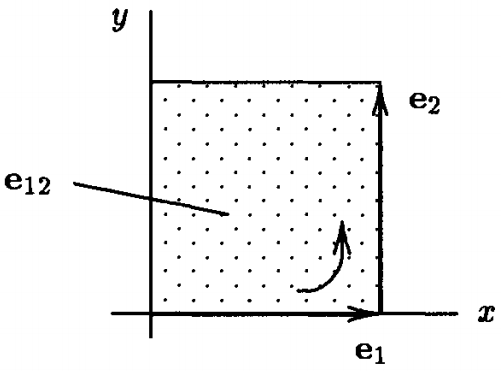
\includegraphics[scale=0.5]{bivetor}
\caption{Representação do bivetor \cite[p. 9]{lounesto2001}}
\label{bivetor}
\end{figure}

\section{A álgebra de Clifford $\Cldois$}\label{algebracl2}

Os quatro elementos 
\[
\begin{array}{rl}
1 & \text{escalar} \\
\vec{e_1}, \vec{e_2} & \text{vetores} \\
\vec{e_{12}} & \text{bivetor}
\end{array}
\]
formam uma base para a álgebra de Clifford $\Cldois$ do plano vetorial $\Rdois$, isto é, um elemento arbitrário
\[
u = u_0 +u_1 \vec{e_1} + u_2\vec{e_2}+ u_{12}\vec{e_{12}} \quad \in \Cldois
\]
é uma combinação linear de um escalar $u_0$, um vetor $u_1 \vec{e_1} + u_2\vec{e_2}$ e um bivetor $u_{12}\vec{e_{12}}$.

A álgebra de Clifford $\Cldois$ é um espaço vetorial real 4-dimensional com elementos da base sendo $1,\vec{e_1}, \vec{e_2}, \vec{e_{12}}$ com a seguinte tábua de multiplicação

\begin{table}[h!]
\centering
\begin{tabular}{c | c c c}
 & $\vec{e_1}$ & $\vec{e_2}$ & $\vec{e_{12}}$\\ \hline
$\vec{e_1}$ & 1 & $\vec{e_{12}}$ & $\vec{e_2}$ \\
$\vec{e_2}$ & $-\vec{e_{12}}$ & 1 & $-\vec{e_1}$ \\
$\vec{e_{12}}$ & $-\vec{e_2}$ & $\vec{e_1}$ & $-1$ 
\end{tabular}
\caption{Tábua de multiplicação de $\Cldois$}
\label{tabuacl2}
\end{table}


\section{O produto exterior}

Extraindo as partes escalar e bivetorial do produto de Clifford temos como produtos de cois vetores $\vec{a}=a_1\vec{e_1}+a_2\vec{e_2}$ e $\vec{b}=b_1\vec{e_1}+b_2\vec{e_2}$
\begin{align*}
\vec{a}\cdot\vec{b}= a_1\vec{b_1}+a_2\vec{b_2}\quad &\text{o produto escalar `$\vec{a}$ ponto $\vec{b}$'}\\
\vec{a}\wedge\vec{b} = \p{a_1b_2-a_2b_1}\vec{e_{12}}\quad &\text{o produto exterior `$\vec{a}$ exterior $\vec{b}$'}
\end{align*}

O bivetor $\vec{a}\wedge\vec{b}$ representa o segmento de plano orientado do paralelogramo com lados $\vec{a}$ e $\vec{b}$. A área desse paralelogramo é $\abs{a_1b_2-a_2b_1}$, e tomaremos como módulo do bivetor $\vec{a}\wedge\vec{b}$ essa área, ou seja, $\abs{\vec{a}\wedge\vec{b}}=\abs{a_1b_2-a_2b_1}$

\begin{figure}[h!]
\centering
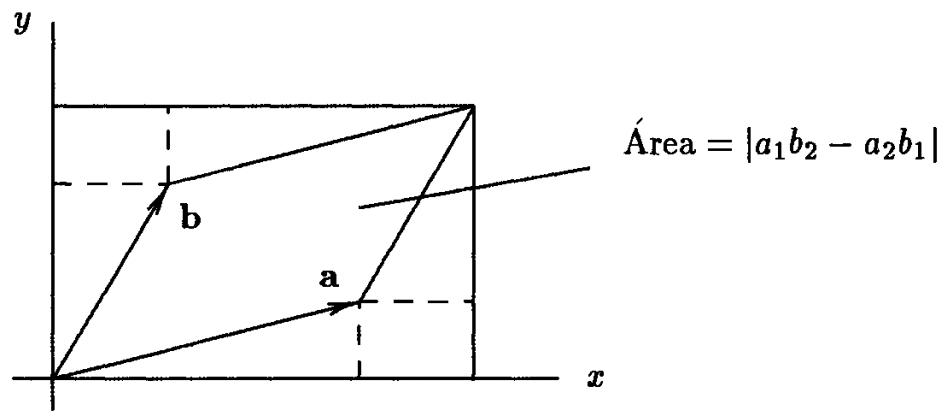
\includegraphics[scale=0.5]{externo}
\caption{Representação do Produto Externo \cite[p. 10]{lounesto2001}}
\label{externo}
\end{figure}

Esse paralelogramo pode ser considerado como um tipo de produto geométrico desses lados

\begin{figure}[h!]
\centering
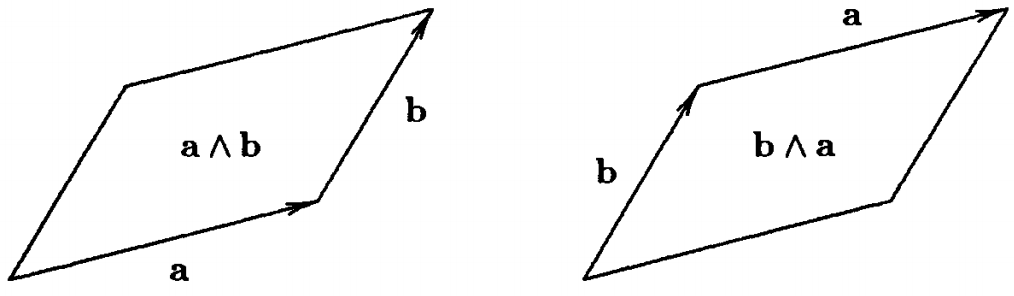
\includegraphics[scale=0.5]{produtogeometrico}
\caption{Representação do Produto Externo \cite[p. 10]{lounesto2001}}
\label{produtogeometrico}
\end{figure}

Os bivetores $\vec{a} \wedge \vec{b}$ e $\vec{b}\wedge\vec{a}$ tem o mesmo módulo (mesma magnitude), mas sentidos de rotação opostos. Assim, podemos expressar essa relação simplesmente por 

\[
\vec{a} \wedge \vec{b} = -\vec{b}\wedge\vec{a}
\]

Usando a tábua de multiplicação da álgebra de Clifford $\Cldois$ [\ref{tabuacl2}], notamos que o produto de Clifford de dois vetores $\vec{a} = a_1\vec{e_1}+a_2\vec{e_2}$ e $\vec{b} = b_1\vec{e_1}+b_2\vec{e_2}$ é 
\begin{align*}
\p{a_1\vec{e_1}+a_2\vec{e_2}}\p{b_1\vec{e_1}+b_2\vec{e_2}} &= a_1\vec{e_1}b_1\vec{e_1}+a_1\vec{e_1}b_2\vec{e_2}+a_2\vec{e_2}b_1\vec{e_1}+a_2\vec{e_2}b_2\vec{e_2} = \\
&=a_1b_1\vec{e_1}\vec{e_1}+a_1b_2\vec{e_1}\vec{e_2}+a_2b_1\vec{e_2}\vec{e_1}+a_2b_2\vec{e_2}\vec{e_2}=\\
&=a_1b_1+a_1b_2\vec{e_12}-a_2b_1\vec{e_12}+a_2b_2=\\
&=a_1b_1+a_2b_2+\p{a_1b_2-a_2b_1}\vec{e_{12}}
\end{align*}

Como $\vec{a} \cdot \vec{b} = a_1b_1+a_2b_2$ e $\vec{a} \wedge \vec{b} = \p{a_1b_2-a_2b_1}\vec{e_{12}}$, podemos reescrever o produto de Clifford como 
\begin{equation}
\vec{ab} = \vec{a} \cdot \vec{b} + \vec{a} \wedge \vec{b} \label{abproduto}
\end{equation}

A propriedade comutativa $\vec{a} \cdot \vec{b} = \vec{b} \cdot \vec{a}$ juntamente com a anticomutatividade $\vec{a} \wedge \vec{b} = -\vec{b} \wedge\vec{a}$ implicam em uma relação entre $\vec{ab}$ e $\vec{ba}$. Então,
\begin{equation}
\vec{ba} = \vec{a} \cdot \vec{b} - \vec{a} \wedge \vec{b} \label{baproduto}
\end{equation}

Somando as equações \ref{abproduto} e \ref{baproduto}, obtemos
\begin{align*}
\vec{ab} + \vec{ba} &= \vec{a} \cdot \vec{b} + \vec{a} \wedge \vec{b} + \vec{a} \cdot \vec{b} - \vec{a} \wedge \vec{b} = \\
&= \vec{a} \cdot \vec{b} + \vec{a} \cdot \vec{b} + \vec{a} \wedge \vec{b} - \vec{a} \wedge \vec{b} = \\
&= 2 \p{\vec{a} \cdot \vec{b}}\\
\vec{a} \cdot \vec{b} &= \frac{1}{2}\p{\vec{ab} + \vec{ba}}
\end{align*}

Subtraindo as equações \ref{abproduto} e \ref{baproduto}, obtemos
\begin{align*}
\vec{ab} - \vec{ba} &= \p{\vec{a} \cdot \vec{b} + \vec{a} \wedge \vec{b}} - \p{\vec{a} \cdot \vec{b} - \vec{a} \wedge \vec{b}}= \\
&= \vec{a} \cdot \vec{b} + \vec{a} \wedge \vec{b}-\vec{a} \cdot \vec{b} + \vec{a} \wedge \vec{b}= \\
&= \vec{a} \cdot \vec{b}-\vec{a} \cdot \vec{b} + \vec{a} \wedge \vec{b} + \vec{a} \wedge \vec{b}= \\
&= 2 \p{\vec{a} \wedge \vec{b}}\\
\vec{a} \wedge \vec{b} &= \frac{1}{2}\p{\vec{ab} - \vec{ba}}
\end{align*}


Dois vetores $\vec{a}$ e $\vec{b}$ são paralelos quando comutam, ou seja, $\vec{ab}=\vec{ba}$ o que implica em $\vec{a}\wedge\vec{b} = 0$; e são ortogonais quando anticomutam, ou seja, $\vec{ab}=-\vec{ba}$ o que implica em $\vec{a} \cdot \vec{b} = 0$. Em resumo,
\begin{align*}
\vec{ab} = \vec{ba} \quad \Longleftrightarrow \quad \vec{a} // \vec{b} \quad \Longleftrightarrow \quad \vec{a}\wedge\vec{b} = 0 \quad \Longleftrightarrow \quad \vec{ab} = \vec{a} \cdot \vec{b} \\
\vec{ab} = -\vec{ba} \quad \Longleftrightarrow \quad  \vec{a} \bot \vec{b} \quad \Longleftrightarrow \quad \vec{a} \cdot \vec{b} = 0 \quad \Longleftrightarrow \quad \vec{ab} =  \vec{a}\wedge\vec{b} \\
\end{align*}

\chapter{Os Números Complexos}\label{complexos}

\section{Definições e propriedades}

\begin{definition}\label{defcomplexos}
Designa-se por conjunto dos números complexos, e representa-se por $\C$, o conjunto $\Rdois$ dos pares ordenados de números reais com a soma vetorial e multiplicação por um escalar usuais, isto é,
\begin{align*}
(x_1,y_1)+(x_2,y_2)&=(x_1+x_2,y_1+y_2)\\
a(x,y)&=(ax,ay)
\end{align*}
e a multiplicação de números complexos definida por
\[
(x_1,y_1)(x_2,y_2)=(x_1x_2 - y_1y_2, x_1y_2 + y_1x_2)
\]
\end{definition}

\begin{obs}O par $(x, 0)$ é identificado com o número real $x$, i. e., 
\[
(x,0)\equiv x
\]

Em outras palavras, temos que $\mathbb{R} \subset \C$. Ao par $(0,1)$ atribuiremos um símbolo, $i$, i. e.,
\[
(0,1) \equiv i
\]
\end{obs}

\subsection*{Consequências}
\begin{enumerate}
\item $z \in \C$, $z=(x,y)=x+yi$, pois
\begin{align*}
x+yi &\equiv (x,0)+(y,0)(0,1) = \\
&= (x,0)+(0,y)=(x,y)
\end{align*}
\item $z=x+yi$ é chamada representação na forma algébrica, onde $x$ é a parte real ($\mathfrak{R}(z)=x$) e $y$ é a parte imaginária ($\mathfrak{I}(z)=y$)
\item $iy = yi$, pois
\[
(0,1)(y,0) = (0,y) = (y,0)(0,1) = yi
\]
\item $i^2 = -1$, pois
\[
(0,1)(0,1)=(-1,0) \equiv -1
\]
\item Dois números complexos dizem-se iguais se, e somente se, tiverem ambos a mesma parte real e a mesma parte imaginária, i. e.,
\[
a+bi=c+di \Leftrightarrow a = c \text{ e } b=d
\]
\item $bi$ é um imaginário puro.
\item Se $z \in \C\bs \{(0,0)\}$ Então, $\exists ! z' \in \C : zz' = 1$
\begin{proof}
Provemos primeiramente a unicidade e, posteriormente, a existência.

\textbf{Unicidade:} Suponhamos que existam $z'$, $z''$ tais que $zz' = 1$ e $zz'' = 1$.

Mas,
\[
z' = z'1 = z'(zz'') = (z'z)z''=1z''=z''
\]
logo, $z'$ é único.

\textbf{Existência:} Seja $z=a+bi \in \C\bs\{(0,0)\}$ e suponhamos $a \neq 0$, no caso $a=0$ vem $z' = - \frac{i}{b}$. Queremos determinar $z'=a'+b'i$ tal que
\[
zz'=1
\]
\begin{align*}
\left\{
\begin{array}{ll}
aa'-bb'&=1\\
ab'+ba'&=0
\end{array}
\right.
&\Leftrightarrow 
\left\{
\begin{array}{ll}
a' = \frac{bb'+1}{a} \\
ab'+b\left(\frac{bb'+1}{a} \right) &= 0
\end{array}
\right. \Leftrightarrow \\
&\Leftrightarrow 
\left\{
\begin{array}{ll}
a' = \frac{bb'+1}{a} \\
a^2b'+b+b^2b'=0
\end{array}
\right. \Leftrightarrow \\
&\Leftrightarrow 
\left\{
\begin{array}{ll}
a' &= \frac{bb'+1}{a} \\
b' &= \frac{-b}{a^2+b^2}
\end{array}
\right. \Leftrightarrow \\
&\Leftrightarrow 
\left\{
\begin{array}{ll}
a' &= \frac{a}{a^2+b^2} \\
b' &= \frac{-b}{a^2+b^2}
\end{array}
\right.
\end{align*}

Assim
\[
z' \equiv z^{-1} = \frac{a}{a^2+b^2} + i \frac{-b}{a^2+b^2}
\]
\end{proof}

\item $\dfrac{z}{w} = zw^{-1} = \dfrac{x+yi}{a+bi} = \dfrac{(x+yi)(a-bi)}{(a+bi)(a-bi)} = \dfrac{xa+yb}{a^2+b^2}+\dfrac{ya-xb}{a^2+b^2}i$
\end{enumerate}

Como consequência das propriedades de $\mathbb{R}$, temos as seguintes propriedades:

\subsection*{Propriedades da adição:}
Para todo $z, w, s \in \C$, segue
\begin{enumerate}[({A}1)]
\item $z+w = w+z$
\item $z+(w+s)=(z+w)+s$
\item $z+0=z$
\item $z+(-z) = 0$
\end{enumerate}

\subsection*{Propriedades da multiplicação:}
Para todo $z, w, s \in \C$, segue
\begin{enumerate}[({M}1)]
\item $zw=wz$
\item $z(ws)=(zw)s$
\item $1z=z$
\item $zz^{-1} = 1$ com $z \in \C\bs\{(0,0)\}$
\end{enumerate}

\subsection*{Lei distributiva:}
\noindent $z(w+s)=zw+zs$, $\forall z, w, s \in \C$

\begin{theorem}
O conjunto dos números complexos constitui um corpo (não ordenado).
\end{theorem}
\begin{proof}
Fica demonstrado observando os seguintes fatos
\begin{enumerate}
\item Em $\C$ não se pode estabelecer uma relação de ordem, pois, se assim
fosse, para uma certa ordem ``$\leq$'' teríamos
\[
i \leq 0 \text{ ou } i \geq 0
\]
mas se $i \leq 0 \Rightarrow i^2 \geq 0 \Leftrightarrow -1 \geq 0$ absurdo, e o mesmo se $i\geq 0$. Assim, não podemos ter uma ordem em $\C$.

\item Podemos estabelecer as propriedades de corpo do conjunto $\C$ a partir do seguinte isomorfismo:

$(\Rdois, \oplus, \otimes)$ é um corpo para $\theta$ e $\phi$ definidas do seguinte modo
\[
(x_1,y_1) \oplus (x_2,y_2):=(x_1+x_2,y_1+y_2)
\]
e
\[
(x_1,y_1) \otimes (x_2,y_2):=(x_1x_2 - y_1y_2, x_1y_2 + y_1x_2)
\]
i. e., $(\Rdois, \oplus)$ e $(\Rdois \bs \{(0,0)\}, \otimes)$ são grupos abelianos.

Define-se
\[
\C:\{z : z=a+bi; a,b \in \mathbb{R}\text{ e } i^2=-1\}
\]
e as seguintes operações em $\C$:
\begin{align*}
(a+bi) +_{\C} (c+di) &:= a+c +i(b+d)\\
(a+bi) \cdot_{\C} (c+di) &:= ac-bd+i(ad+bc)\\
\end{align*}

Seja
\[
f : \Rdois \rightarrow \C, \,\,(x,y) \mapsto x+yi
\]

$f$ é um isomorfismo de $(\Rdois, \oplus, \otimes)$ sobre $(\C, +_{\C}, \cdot_{\C})$, i. e., uma transformãção que trasforma a operação $\theta$ na operação $+_{\C}$ e a operação $\phi$ na operação $\cdot_{\C}$. Para simplificar a notação e por abuso de linguagem, representa-se $+_{\C}$ por $+$ e $\cdot_{\C}$ por $\cdot$.
\end{enumerate}
\end{proof}

\begin{proposition}
Seja $z \in \C$. Então existe $w \in \C$ tal que $w^2 = z$. O corpo $\C$ é a menor extensão de $\mathbb{R}$ onde $w^2=z$ tem sempre solução. Notemos que $-w$ também satisfaz a equação. \label{prop5}
\end{proposition}

\begin{proof}
Seja $z=a+bi$ Pretendemos encontrar $w=x+yi$ tal que 
\[
a+bi = (x+yi)^2 \Leftrightarrow \left\{\begin{array}{ll}
x^2-y^2=a\\
2xy=b
\end{array}
\right.
\]

Temos
\begin{align*}
a^2+b^2 &= (x^2-y^2)^2+4x^2y^2=(x^2+y^2)^2 \Leftrightarrow\\
&\Leftrightarrow x^2+y^2 = \sqrt{a^2+b^2} \Leftrightarrow\\
&\Leftrightarrow -a+x^2+x^2=\sqrt{a^2+b^2} \Leftrightarrow\\
&\Leftrightarrow x^2 = \frac{1}{2} \left(a+\sqrt{a^2+b^2}\right) \text{ e } y^2 = \left(-a+\sqrt{a^2+b^2}\right)
\end{align*}

Seja
\[
\alpha = \sqrt{\frac{1}{2} \left(a+\sqrt{a^2+b^2}\right)} \text{ e } \beta = \sqrt{\frac{1}{2} \left(-a+\sqrt{a^2+b^2}\right)}
\]
\begin{enumerate}
\item $b>0$: $(x=\alpha \text{ e } y=\beta) \vee (x=-\alpha \text{ e } y=-\beta)$
\item $b<0$: $(x=-\alpha \text{ e } y=\beta) \vee (x=\alpha \text{ e } y=-\beta)$
\end{enumerate}

Concluimos, pois, que, para $b>0$, temos
\[
\left\{\begin{array}{ll}
x &=\sqrt{\frac{1}{2} \left(a+\sqrt{a^2+b^2}\right)}\\
y &=\sqrt{\frac{1}{2} \left(-a+\sqrt{a^2+b^2}\right)}
\end{array}
\right.
\vee
\left\{\begin{array}{ll}
x &=-\sqrt{\frac{1}{2} \left(a+\sqrt{a^2+b^2}\right)}\\
y &=-\sqrt{\frac{1}{2} \left(-a+\sqrt{a^2+b^2}\right)}
\end{array}
\right.
\]
e, para $b<0$, temos
\[
\left\{\begin{array}{ll}
x &=-\sqrt{\frac{1}{2} \left(a+\sqrt{a^2+b^2}\right)}\\
y &=\sqrt{\frac{1}{2} \left(-a+\sqrt{a^2+b^2}\right)}
\end{array}
\right.
\vee
\left\{\begin{array}{ll}
x &=\sqrt{\frac{1}{2} \left(a+\sqrt{a^2+b^2}\right)}\\
y &=-\sqrt{\frac{1}{2} \left(-a+\sqrt{a^2+b^2}\right)}
\end{array}
\right.
\]
\end{proof}

\section{Complexos conjugados}

\begin{definition}
Dado $z = x + yi \in \C$, designa-se por conjugado de $z$, ao número complexo $\overline{z}=x-yi$, i. e., é uma simetria do ponto $z$ em relação ao eixo $x$
\end{definition}

\section*{Consequências}
Para todo $z_1$ e $z_2 \in \C$
\begin{enumerate}
\item $\overline{z_1+z_2} = \overline{z_1}+\overline{z_2}$
\item $\overline{z_1\cdot z_2} = \overline{z_1}\cdot \overline{z_2}$
\item $\overline{\dfrac{z_1}{z_2}} = \dfrac{\overline{z_1}}{\overline{z_2}}$, com $z_2 \in \C \bs \{(0,0)\}$
\item $z=\overline{z} \Leftrightarrow z \in \mathbb{R}$
\item $z+\overline{z}= 2\mathfrak{R}(z) \text{ e } z - \overline{z}=2i\mathfrak{I}(z)$
\end{enumerate}

\section{Valor absoluto}

\begin{definition}
Dado $z= x+yi \in \C$, chama-se valor absoluto de $z$, ao número real não negativo
\[
\abs{z}= \sqrt{x^2+y^2}
\]

Geometricamente $\abs{z}$ é o comprimento do vetor $(x,y)$
\end{definition}

\begin{proposition}
Para quaisquer $z, z_1, z_2 \in \C$ temos \label{prop9}
\begin{enumerate}
\item $\abs{z}^2 = (\mathfrak{R}(z))^2+(\mathfrak{I}(z))^2$
\item $\abs{z}> \abs{\mathfrak{R}(z)}$ e $\abs{z} \geq \abs{\mathfrak{I}(z)}$
\item $z\overline{z}=x^2+y^2=\abs{z}^2$, $\abs{\overline{z}}=\abs{z}$, $z^{-1} = \dfrac{\overline{z}}{\abs{z}^2}$
\item $\abs{z_1z_2}=\abs{z_1}\abs{z_2}$
\item $\abs{\dfrac{z_1}{z_2}}=\dfrac{\abs{z_1}}{\abs{z_2}}$, $z_2 \neq 0$
\item $\abs{z_1+z_2}<\abs{z_1}+\abs{z_2}$ (desigualdade triangular)
\item $\abs{z_1-z_2}\geq \abs{\abs{z_1}-\abs{z_2}}$
\end{enumerate}
\end{proposition}

\begin{proof}
Deixamos as demonstrações dos itens da \propositionref{prop9} como exercício para o leitor.
\end{proof}

\section{Forma polar}
Para cada número complexo $z=x+yi \in \C \bs \{0\}$, podemos associar as suas coordenadas polares $r$ e $\theta$, dadas por:
\[
r = \abs{z} = \sqrt{x^2+y^2}
\]
\[
\theta = \arg z = \arctan \frac{y}{x} \text{, } 0 \leq \theta \leq 2\pi
\]

Assim, 
\[
\left\{\begin{array}{ll}
x= r \cos \theta\\
y= r \sin \theta
\end{array}
\right.
\quad r>0 \text{, } \theta \in [0, 2\pi[
\]
pelo que podemos escrever
\begin{notation}
$z=x+yi \Leftrightarrow z=r(\cos \theta + i \sin \theta)$. Esta é a representação de $z$ na forma polar.
\end{notation}

\begin{obs}
Para cada $z \in \C$, $\arg z$ não é único, na verdade, dado que $\sin \theta$ e $\cos \theta$ são funções periódicas de período $2\pi$, se $\theta$ é o argumento de $z$, então $\theta +2k\pi$, ($k \in \mathbb{Z}$) também o é. No entanto, se fixarmos um intervalo $\theta_0 \leq \arg z < \theta_0+2\pi$ a representação é única. Também segue que $\arg z = -\arg\overline{z}$
\end{obs}

\begin{theorem}
Dados $z_1,z_2 \in \C$ com $z_1 = r_1(\cos\theta_1+i\sin\theta_1)$ e $z_2 = r_2(\cos\theta_2+i\sin\theta_2)$, então $z_1z_2=r_1r_2(cos(\theta_1+\theta_2)+i\sin(\theta_1+\theta_2))$, i.e., 
\[
\abs{z_1z_2}=\abs{z_1}\abs{z_2}
\]
e
\[
\arg(z_1z_2) = \arg z_1 + \arg z_2 (\text{mod } 2\pi)
\] \label{teo12}
\end{theorem}
\begin{proof}
Basta multiplicar os números complexos com a representação na forma polar e usar as fórmulas trigonométricas
\[
\cos\theta_1\cos\theta_2-\sin\theta_1\sin\theta_2 = \cos(\theta_1+\theta_2)
\]
e
\[
\sin\theta_1\cos\theta_2+\cos\theta_1\sin\theta_2 = \sin(\theta_1+\theta_2)
\]
\end{proof}

\section{A álgebra real $\C$}

É compreendível a ideia de tomar $\R$ como um único subcorpo em $\C$. Porém, $\C$ contém muitos subcorpos isomorfos a $\R$; escolher um significa introduzir uma estrutura linear real em $\C$, obtendo por restrição $a$ no produto $\C \times \C \to \C$, $(a,b)\to ab$ ser real, $a \in \R$. Tal estrutura torna o corpo $\C$ em uma álgebra real $\C$

Afim de distinguir o corpo $\C$ da álgebra real $\C$, construamos, como em \definitionref{defcomplexos}, porém sem a multiplicação com escalar definida. Assim $\C$ é construído como o conjunto $\R \times \R$ de todos os pares ordenados de números reais $z=(x,y)$ com soma e multiplicação definidos.

O conjunto $\R \times \R$ juntamente com a tais soma e multiplicação configuram o corpo $\C$. A unidade imaginária $(0,1)$ satisfaz $(0,1)^2=(-1,0)$.

Visto que $(x_1,0)+(x_2,0)=(x_1+x_2,0)$ e $(x_1,0)(x_2,0)=(x_1x_2,0)$, o corpo real $\R$ está contido em $\C$ como um subcorpo $\R \to \C$, $x \to (x,0)$. Se restringirmos a multiplicação de modo que esse fator esteja nesta cópia distinta de $\R$,
\[
(\lambda,0)(x,y)=(\lambda x,\lambda y)
\]
assim introduzimos uma estrutura linear real no conjunto $\Rdois = \R \times \R$. Esta estrutura linear real nos permite visualizar o corpo $\C$ intuitivamente como o plano complexo $\C$. 

A construção acima de $\C$ como um espaço linear real $\Rdois$ traz mais estrutura que apenas a estrutura de corpo, essa construção torna $\C$ uma álgebra sobre $\R$. Nós podemos identificar $\R$ com o subcorpo $\chaves{(x,0) | x \in \R}$ de $\C$ e denotar as base canônica de $\Rdois$ por $1=(1,0)$, $i=(0,1) \in \C$.

\begin{definition}
Uma aplicação $\alpha: \C \to \C$ é um automorfismo do corpo $\C$ se preservar a adição e a multiplicação, i. ie.
\begin{align*}
&\alpha\p{z_1+z_2} = \alpha z_1 + \alpha z_2 \\
&\alpha\p{z_1z_2} = \alpha(z_1)\alpha(z_2)
\end{align*}
bem como a unidade, $\alpha(1)=1$.
\end{definition}

\begin{definition}
Uma aplicação $\alpha: \C \to \C$ é um automorfismo da álgebra real $\C$ se preservar a estrutura linear real e a multiplicação (dos números complexos), i. e. 
\begin{align*}
&\alpha\p{z_1+z_2} = \alpha z_1 + \alpha z_2, \quad \alpha(\lambda z) = \lambda \alpha(z), \quad \lambda \in \R \\
&\alpha\p{z_1z_2} = \alpha(z_1)\alpha(z_2)
\end{align*}
bem como a unidade, $\alpha(1)=1$.
\end{definition}

O corpo $\C$ tem infinitos automorfismos. Entretanto, os únicos automorfismo da álgebra real $\C$ são a identidade e a conjugação complexa.

\chapter{Partes da álgebra de Clifford $\Cldois$}\label{partesdecl2}

\section{$\C$ como a parte par da álgebra de Clifford $\Cldoispar$}\label{ccomopartedecldois}

Como vimos em \ref{algebracl2}, a álgebra de Clifford $\Cldois$ é uma álgebra real 4-dimensional com uma de suas bases $\chaves{1, \vec{e_1}, \vec{e_2}, \vec{e_{12}}}$. Os elementos da base geram os subespaços
\[
\begin{array}{rcl}
1& \R & \text{escalar} \\
\vec{e_1}, \vec{e_2}& \Rdois & \text{vetores} \\
\vec{e_{12}}& \bigwedge^2 \Rdois & \text{bivetor}
\end{array}
\]

Portanto, a álgebra de Clifford $\Cldois$ contém cópias de $\R$ e $\Rdois$ e é uma soma direta desses subespaços de elementos de grau 0,1,2; i. e.
\[
\Cldois = \R \oplus \Rdois \oplus \bigwedge^2 \Rdois
\]

Também podemos escrever 
\[
\Cldois = \Cldoispar \oplus \Cldoisimpar
\]
onde 
\[
\begin{array}{rl}
\text{parte par}& \Cldoispar = \R \oplus \bigwedge^2 \Rdois\\
\text{parte impar}& \Cldoisimpar = \Rdois 
\end{array}
\]


\begin{proposition}\label{subalgebracldoispar}
A parte par $\Cldoispar$ é uma subálgebra de $\Cldois$
\end{proposition}
\begin{proof}
Basta demonstrar-mos que $\Cldoispar$ é fechada em relação ao produto de Clifford de $\Cldois$. Dados $\p{x_1+y_1\vec{e_{12}}}$ e $\p{x_2+y_2\vec{e_{12}}} \in \Cldoispar$, o produto de Clifford é 
\[
\p{x_1+y_1\vec{e_{12}}}\p{x_2+y_2\vec{e_{12}}} = \p{x_1x_2-y_1y_2}+\p{x_1y_2+x_2y_1}\vec{e_{12}} \in \Cldoispar
\]
\end{proof}

Da \propositionref{subalgebracldoispar}, concluímos que a parte par não é somente um subespaço mas também uma subálgebra. Esta parte consiste de elementos da forma $x+y\vec{e_{12}}$ onde $x, y \in \R$ e $\vec{e_{12}}^2 = -1$. Portanto, a subálgebra par $\Cldoispar = \R \oplus \bigwedge^2 \R^2$ de $\Cldois$ é isomorfo a $\C$. O bivetor unitário $\vec{e_{12}}$ compartilha a propriedade básica da raiz quadrada $i$ de $-1$, i. e. $i^2= -1$, de modo que podemos escrever $i=\vec{e_{12}}$.

Notemos que a unidade imaginária $\vec{e_{12}}$ anticomuta com $\vec{e_1}$ e $\vec{e_2}$, portanto $\vec{e_{12}}$ anticomuta com todos os vetores no plano $\vec{e_1}\vec{e_2}$.

\section{As partes par e ímpar de $\Cldois$}

Como visto em \ref{ccomopartedecldois}, a álgebra de Clifford $\Cldois$ contém ambos os planos complexo ($\C$) e real ($\Rdois$), de modo que 
\[
\begin{array}{ll}
\Rdois & \text{é gerado por } \vec{e_1} \text{ e } \vec{e_2}\\
\C & \text{é gerado por } 1 \text{ e } \vec{e_{12}}
\end{array}
\]

O único ponto em comum desses planos é o $0$. Ambos os planos são partes da mesma álgebra $\Cldois$. O plano vetorial $\Rdois$ e o corpo complexo $\C$ são incorporados como subestruturas separadas na álgebra de Clifford, de modo que o plano complexo $\C$ é a parte par $\Cldoispar$ e o plano vetorial $\Rdois$ é a parte ímpar $\Cldoisimpar$.

Os nomes par e ímpar significam que os elementos são produtos de um número par ou ímpar de vetores. Considerações sobre paridade, mostram que 
\begin{enumerate}[i.]
\item o produto de números complexos é um complexo;
\item o produto de um vetor por um complexo é um vetor;
\item o produto de um complexo por um vetor é um vetor e
\item o produto de vetores é um número complexo.
\end{enumerate}

Tais observações podem ser expressas por 
\begin{align*}
\Cldoispar\Cldoispar &\subset \Cldoispar ,\\
\Cldoisimpar\Cldoispar &\subset \Cldoisimpar, \\
\Cldoispar\Cldoisimpar &\subset \Cldoisimpar, \\
\Cldoisimpar\Cldoisimpar &\subset \Cldoispar.
\end{align*}

Escrevendo $\p{\Cldois}_0 = \Cldoispar$ e $\p{\Cldois}_1 = \Cldoisimpar$, podemos resumir as inclusões acima como 
\[
\p{\Cldois}_j\p{\Cldois}_k \subset \p{\Cldois}_{j+k}
\]
onde $j$ e $k$ são adicionados módulo 2.

Essas observações são expressas dizendo que a álgebra de Clifford $\Cldois$ tem graduação par-ímpar ou que é $\mathbb{Z}_2$-graduada.
% ---
% Finaliza a parte no bookmark do PDF, para que se inicie o bookmark na raiz
% ---
\bookmarksetup{startatroot}% 
% ---

% ----------------------------------------------------------
% Conclusão
% ----------------------------------------------------------
\chapter{Conclusão}


% ----------------------------------------------------------
% ELEMENTOS PÓS-TEXTUAIS
% ----------------------------------------------------------
\postextual


% ----------------------------------------------------------
% Referências bibliográficas
% ----------------------------------------------------------
\bibliography{ref-algebrasdeclifford}


% ----------------------------------------------------------
% Apêndices
% ----------------------------------------------------------
%\begin{apendicesenv}
%\chapter{Quisque libero justo}
%\lipsum[50]
%
%\chapter{Nullam elementum urna vel imperdiet sodales}
%\lipsum[55-57]
%\end{apendicesenv}


% ----------------------------------------------------------
% Anexos
% ----------------------------------------------------------
%\begin{anexosenv}
%
%\chapter{Morbi ultrices rutrum lorem.}
%\lipsum[30]
%
%\chapter{Fusce facilisis lacinia dui}
%\lipsum[32]
%
%\end{anexosenv}

% ----------------------------------------------------------
% FIM DO DOCUMENTO
% ----------------------------------------------------------
\end{document}